\setlength{\parindent}{2em}

\chapter{Simulation \& Validation}
    \section{Simulation}
    \noindent
    Before packaging into IP and system-level integration, the RTL design is tested on some data to ensure the data and control units are working properly and give the desired result from the convolution operation. 

    \noindent The following kernel is chosen for simulation purposes, and the bias value is taken as:
    
    \begin{center}
    \begin{tabular}{|c|c|c|}
    \hline
    -0.03322114422917366 & -0.18549901247024536 & -0.25089457631111145 \\ \hline
    0.025202458724379539 & 0.15725375711917877 & 0.044544823467731476 \\ \hline
    0.20101584494113922 & 0.072924628853797913 & 0.24815583229064941 \\ \hline
    \end{tabular}
    \end{center}
    

    \[
    \text{bias} = -0.04632568359375
    \]

    \begin{table}[h]
    \centering
    \begin{tabular}{|c|c|}
        \hline
        \textbf{Decimal Representation} & \textbf{16-bit Fixed Representation} \\
        \hline
        -0.03322114422917366 & 1\_111\_111101110111 \\
        \hline
        -0.18549901247024536 & 1\_111\_110100000111 \\
        \hline
        -0.25089457631111145 & 1\_111\_101111111011 \\
        \hline
        0.025202458724379539 & 0\_000\_000001100111 \\
        \hline
        0.15725375711917877  & 0\_000\_001010000100 \\
        \hline
        0.044544823467731476 & 0\_000\_000010110110 \\
        \hline
        0.20101584494113922  & 0\_000\_001100110111 \\
        \hline
        0.072924628853797913 & 0\_000\_000100101010 \\
        \hline
        0.24815583229064941  & 0\_000\_001111111000 \\
        \hline
        -0.04632568359375 & 1\_111\_111101000010 \\
        \hline
    \end{tabular}
    \caption{Decimal and 16-bit Fixed-Point Representation of 3×3 Kernel Values and Bias}
    \label{tab:fixed_point}
\end{table}

    \subsection{Convolution Simulation}
    \noindent The table \ref{tab:fixed_point} shows the representation of kernel weights and bias in the adopted 16-bit fixed point representation standard. The \textit{underscore} is used to separate the respective fields(sign, integer, fraction) from one another. 

    \noindent 
    Figure \ref{fig:conv_tb_simulation} shows the simulation performed on some sample image, some of the data points seen on the simulator are results of the convolution operation on the first image row. 

    \begin{figure}
        \centering
        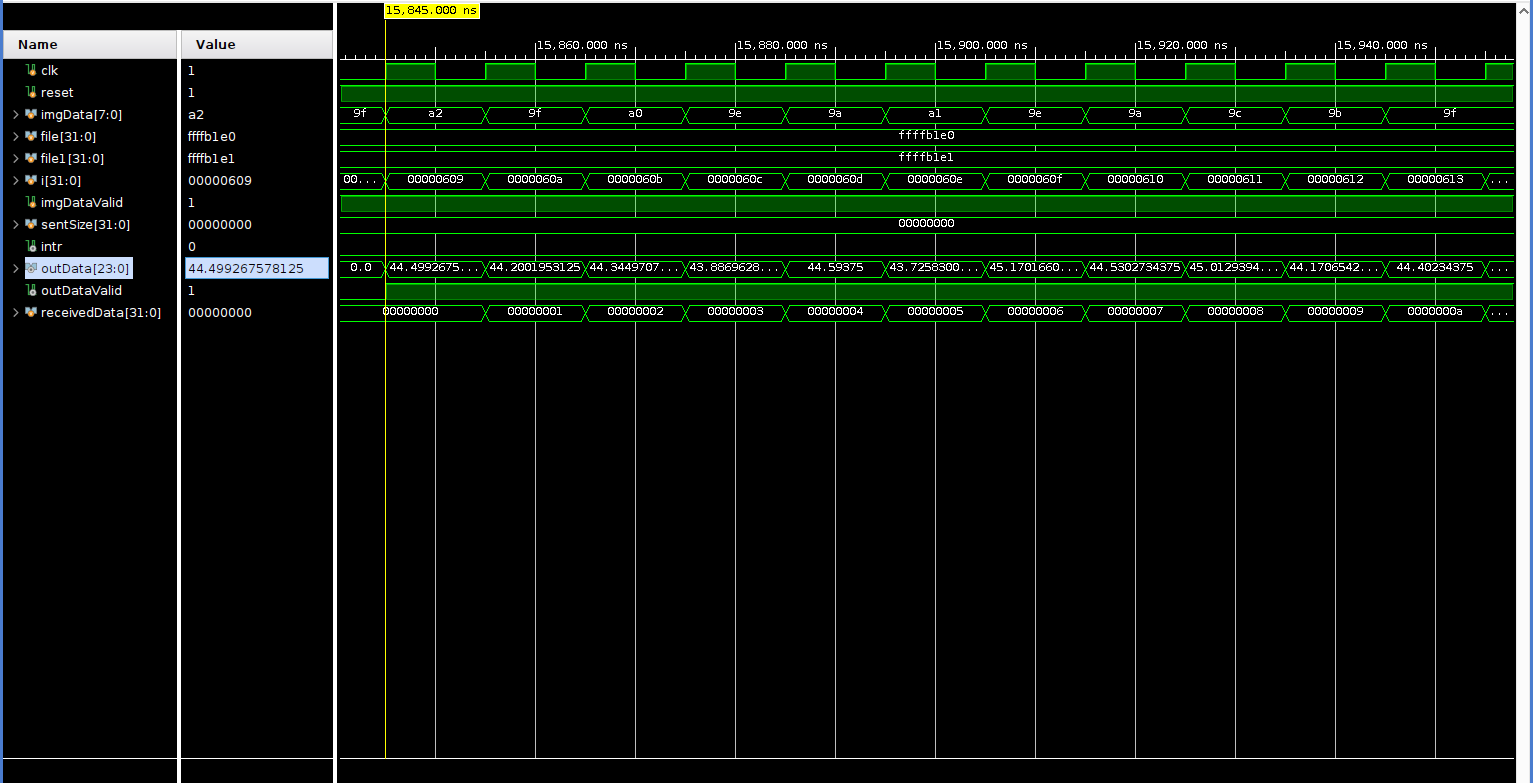
\includegraphics[width=1\linewidth]{images/simulationWaveform.png}
        \caption{Convolution Simulation}
        \label{fig:conv_tb_simulation}
    \end{figure}

    \begin{table}[ht]
    \centering
    \begin{tabular}{|c|c|c|}
        \hline
        \textbf{Input Data Stream} & \textbf{Obtained Output} & \textbf{Decimal} \\
        \hline
        0xA0A0A0A1A09FA0A1A0 & 44.499267578125 & 44.724472 \\
        0xA0A09FA09F9FA1A09E & 44.2001953125 & 44.424690 \\
        0xA09FA19F9FA1A09EA1 & 44.344970703125 & 44.569893 \\
        0x9FA19C9FA19B9EA19C & 43.886962890625 & 44.109791 \\
        0xA19CA1A19BA1A19CA2 & 44.59375 & 44.817875 \\
        0x9CA19F9BA19F9CA29F & 43.725830078125 & 43.949493 \\
        0xA19FA2A19FA3A29FA3 & 45.170166015625 & 45.396538 \\
        0x9FA29F9FA39F9FA39F & 44.5302734375 & 44.755623 \\
        0xA29FA0A39FA0A39FA0 & 45.012939453125 & 45.238426 \\
        0x9FA09E9FA09E9FA09E & 44.170654296875 & 44.394283 \\
        \hline
    \end{tabular}
    \caption{Convolution Operation input data, obtained output, and actual output}
    \label{tab:data_stream}
\end{table}

    \noindent The table \ref{tab:data_stream} shows the set of input and output for one 3x3 pixel data in the first column which is 72 bits wide the second column shows obtained output in its equivalent 16-bit fixed point representation adopted in this project, and the last column shows the expected convolution operation result in decimal. The results shown in the \ref{tab:data_stream} are also observed waveform window during the simulation as shown in the figure \ref{fig:conv_tb_simulation}. The figure shows the golden data for comparison, which is seen on \textit{MATLAB}, the first window shows image pixel data, and the second window shows the convolution operation along with added bias.

    \begin{figure}
        \centering
        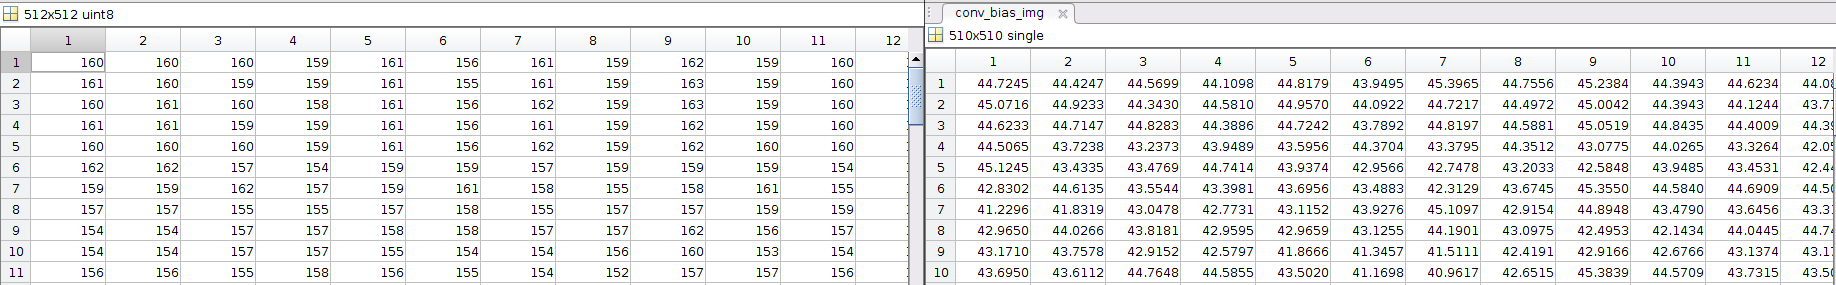
\includegraphics[width=1\textwidth]{images/matlabGoldenData.png}
        \caption{Matlab golden data for Convolution operation}
        \label{fig:matlabGoldenData}
    \end{figure}
    
    \par
    \noindent Now, from the obtained output for a given input, it can be seen that these values are nearly the same when compared to the expected output, the difference is mainly because while adopting a 16-bit fixed point standard from a float32, some precision is lost.

    \subsection{Maxpool Simulation}
    \noindent
    The maxpool logic involves no arithmetic operations and comprises comparison as the only operation thus, whether the maximum value from the appropriate window is obtained is the only point to be verified.
    Figures \ref{fig:convWindow1} and  \ref{fig:convWindow2} represent output convolved data when the convolution kernel is convoluted on the first and the second row. 
    \begin{figure}
        \centering
        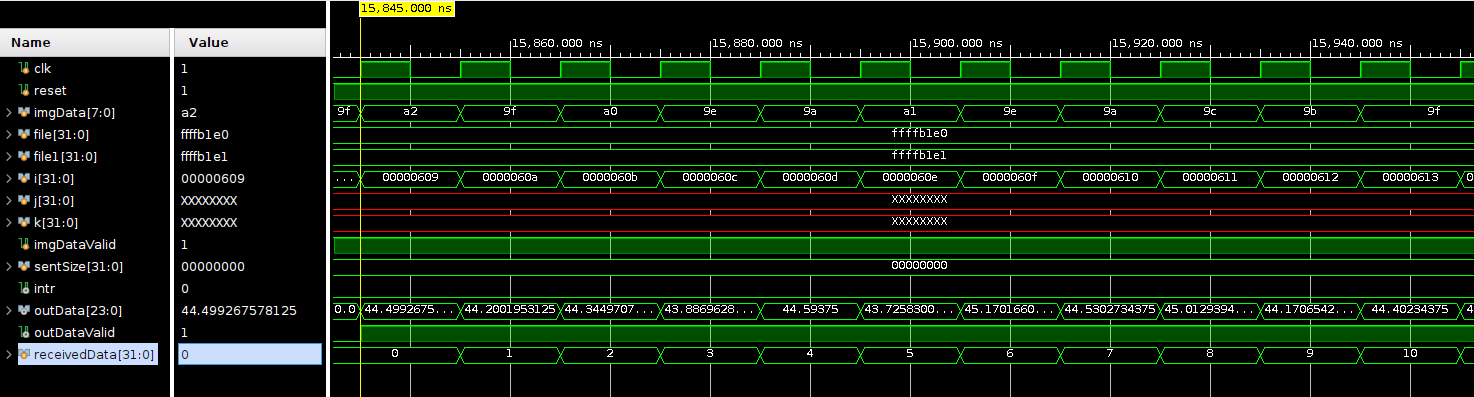
\includegraphics[width=\linewidth]{images/convWindow1.png}
        \caption{Convolution first row output on Vivado Simulator}
        \label{fig:convWindow1}
    \end{figure}
    \begin{figure}
        \centering
        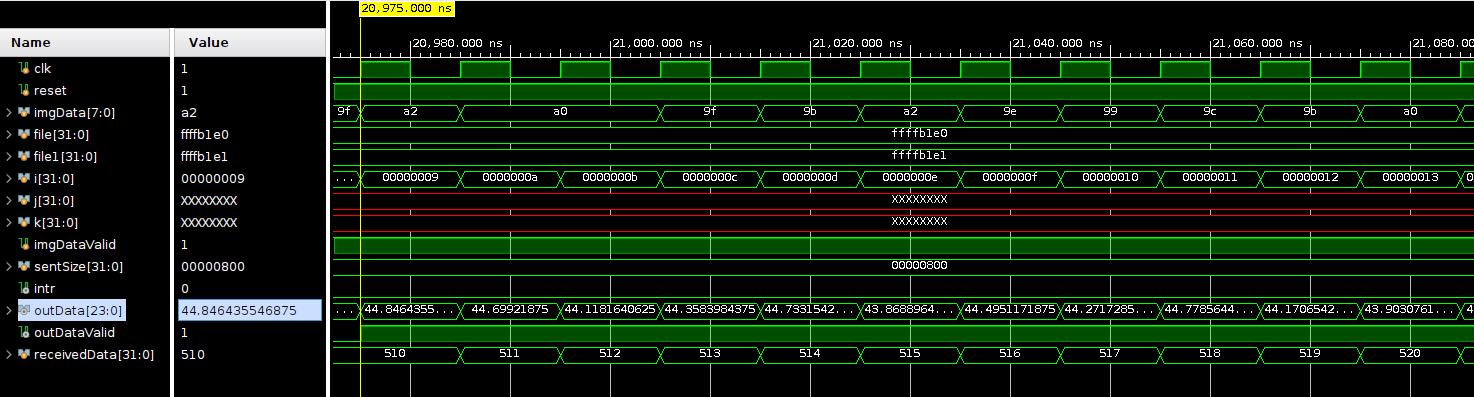
\includegraphics[width=\linewidth]{images/convWindow2.png}
        \caption{Convolution second row output on Vivado Simulator}    
        \label{fig:convWindow2}
    \end{figure}

    \noindent
    Figure \ref{fig:maxpoolrow1} shows the max-pooled output when the kernel is applied on the first two rows(kernel size of 2x2) of convolved data with a stride of 2. For comparison with reference data, figure \ref{fig:matlabMaxpool} shows reference maxpool and convolution data.

    \begin{figure}
        \centering
        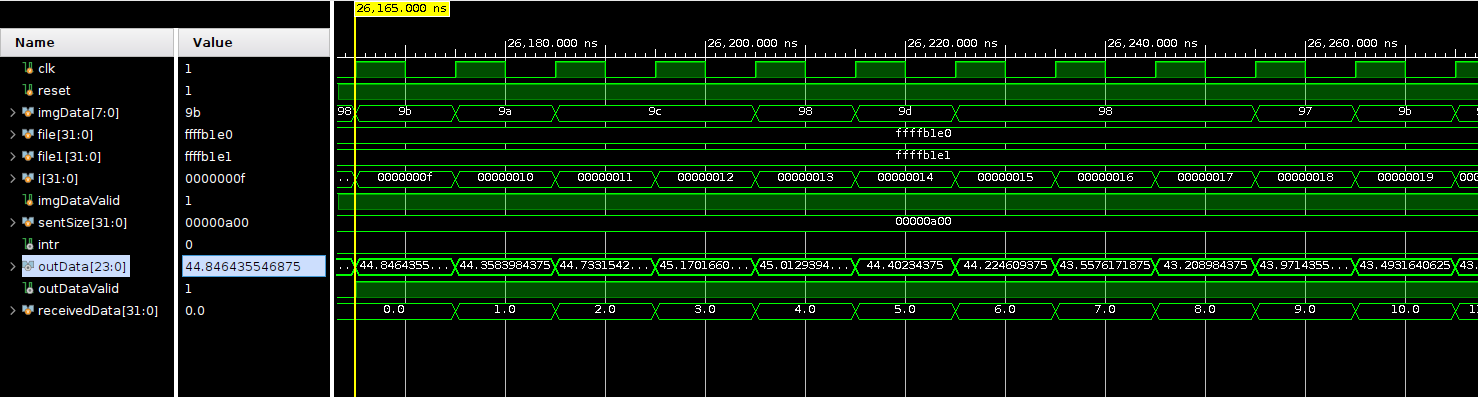
\includegraphics[width=\linewidth]{images/maxpoolRow1.png}
        \caption{Maxpool first row output on Vivado Simulator}
        \label{fig:maxpoolrow1}
    \end{figure}

    \begin{figure}
        \centering
        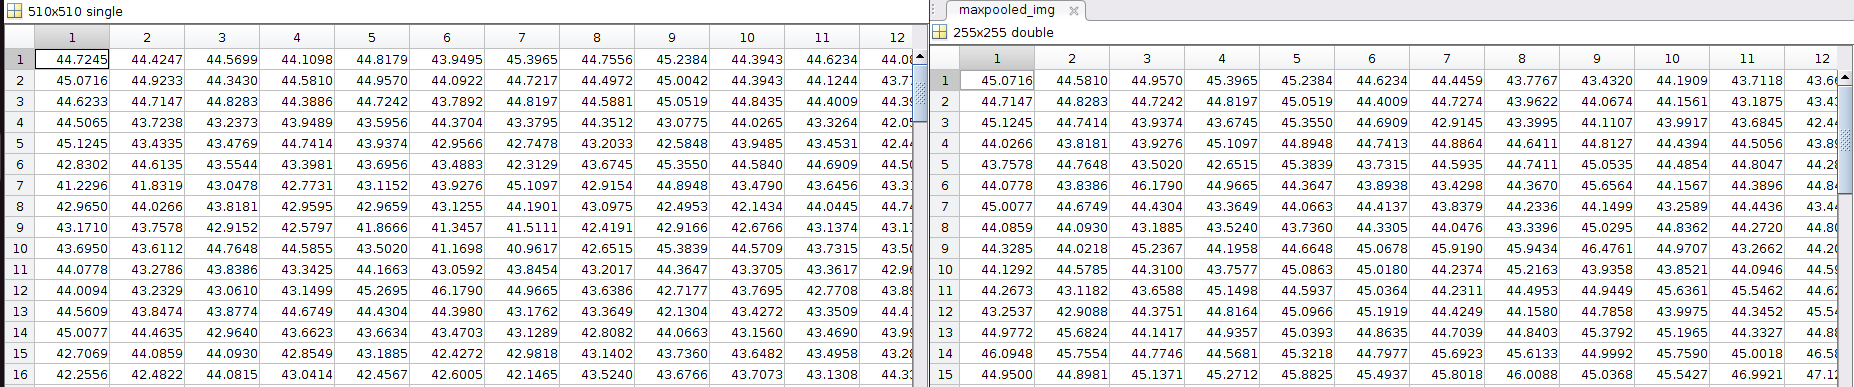
\includegraphics[width=\linewidth]{images/matlabConvMaxRefdata.png}
        \caption{Matlab reference convolution and Maxpool data}
        \label{fig:matlabMaxpool}
    \end{figure}
    
    
    \section{Validation}
    \noindent
    During the initial phase of design and development, it is necessary to evaluate the functionality of the design at the Hardware level, knowing that FPGA-based systems are very critical while implementing on actual hardware. Once the scale of design is increased, it may be difficult to find the bugs and debug the design. Thus, in the initial phase, a hardware-level evaluation is carried out.
    \subsection{Convolution IP Hardware Level Evaluation}
    \noindent
    After the simulation, once the RTL's functionality is verified, the convolution logic is packaged as an IP using the Vivado IP packager tool, and the IP is based on the AXI4 Stream protocol. To receive the image, the PS is programmed to receive the image through the UART interface. The PS is provided with the hardware configuration using an XSA(Xilinx Specification Archive) file. The PS is also programmed to transfer the received image using the DMA to the convolution IP(topConv). A system-level check is performed where the system only performs a convolution operation. The main reason to only perform testing on the Convolution IP is to keep the debug process simple. This acts like an initial testing to check whether, at the hardware level does the data is being received properly by the FPGA through the UART. The system-level block diagram is shown in Figure \ref{fig:block-design}. This design also includes a debug core, which can be seen in the block design by the name \textit{System ILA}, which helps observe the waveforms when the actual evaluation of the logic is performed on the board. The debug core enables observing waveforms at the actual hardware level, and can be seen on Vivado. 

    \begin{figure}[H]
        \centering
        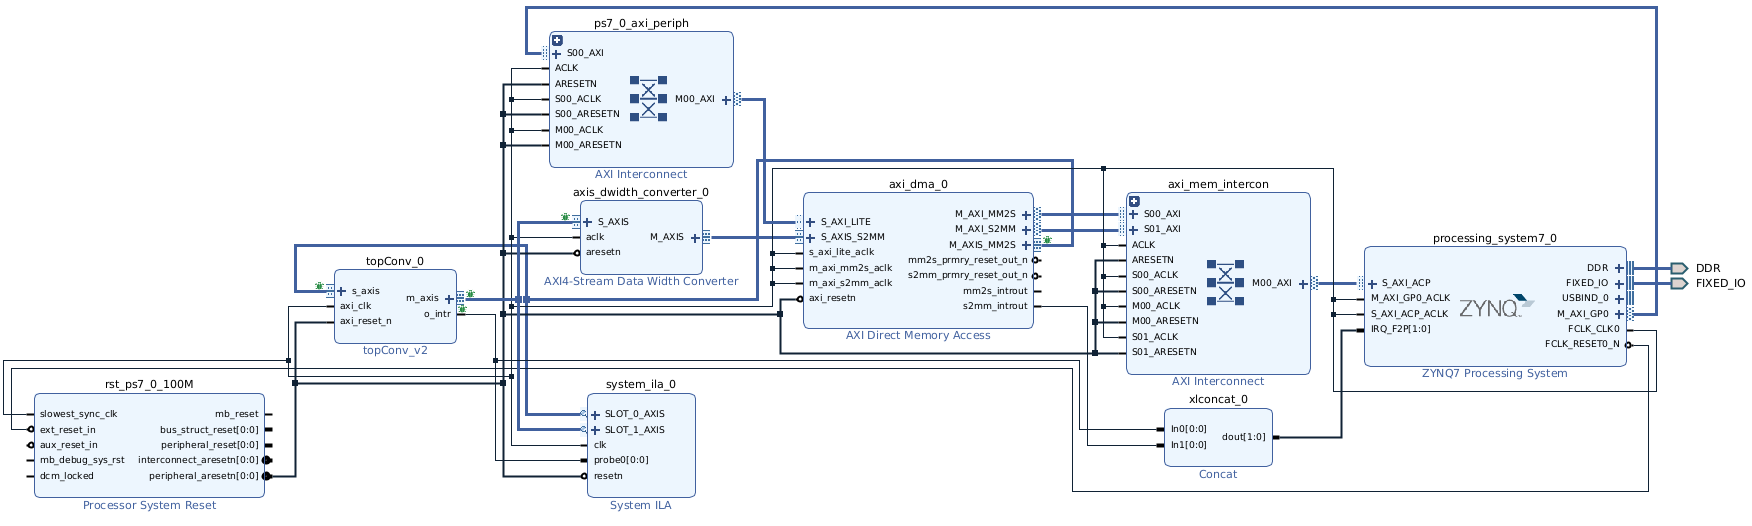
\includegraphics[width=\linewidth]{images/BlockDesign.png}
        \caption{Convolution IP system level block diagram in Vivado}
        \label{fig:block-design}
    \end{figure}
    
    \noindent Steps Involved:
    \begin{enumerate}[noitemsep, topsep=3pt]
        \item Open Hardware Manager in Vivado, connect to the PYNQ-Z2 board
        \item Setup a trigger after which samples are to be collected
        \item Using the Vitis IDE program, the PS 
        \item In Vivado, click on \textit{refresh device} and then program the device
        \item Using Teraterm, set a serial connection between the PC and PYNQ-Z2 
        \item In Vivado, run the trigger 
        \item Using Teraterm, send the image in binary format
        \item Observe waveforms generated from debug cores on Vivado
    \end{enumerate}

    \noindent
    Figures \ref{fig:dmaTrigger} and \ref{fig:convDataTrigger} show the triggers which have been setup, as can be seen in the Trigger setup window appearing at the bottom right corner. The triggers start to sample signals whenever \textit{valid} signal goes low-to-high. Here, triggers have been setup for mainly two tasks:

    \begin{enumerate}[noitemsep, topsep=3pt]
        \item Check whether appropriate Image data is transferred by DMA to the Convolution IP
        \item Check if convoluted data is being transferred from Convolution IP to DMA
    \end{enumerate}

    \begin{figure}[H]
        \centering
        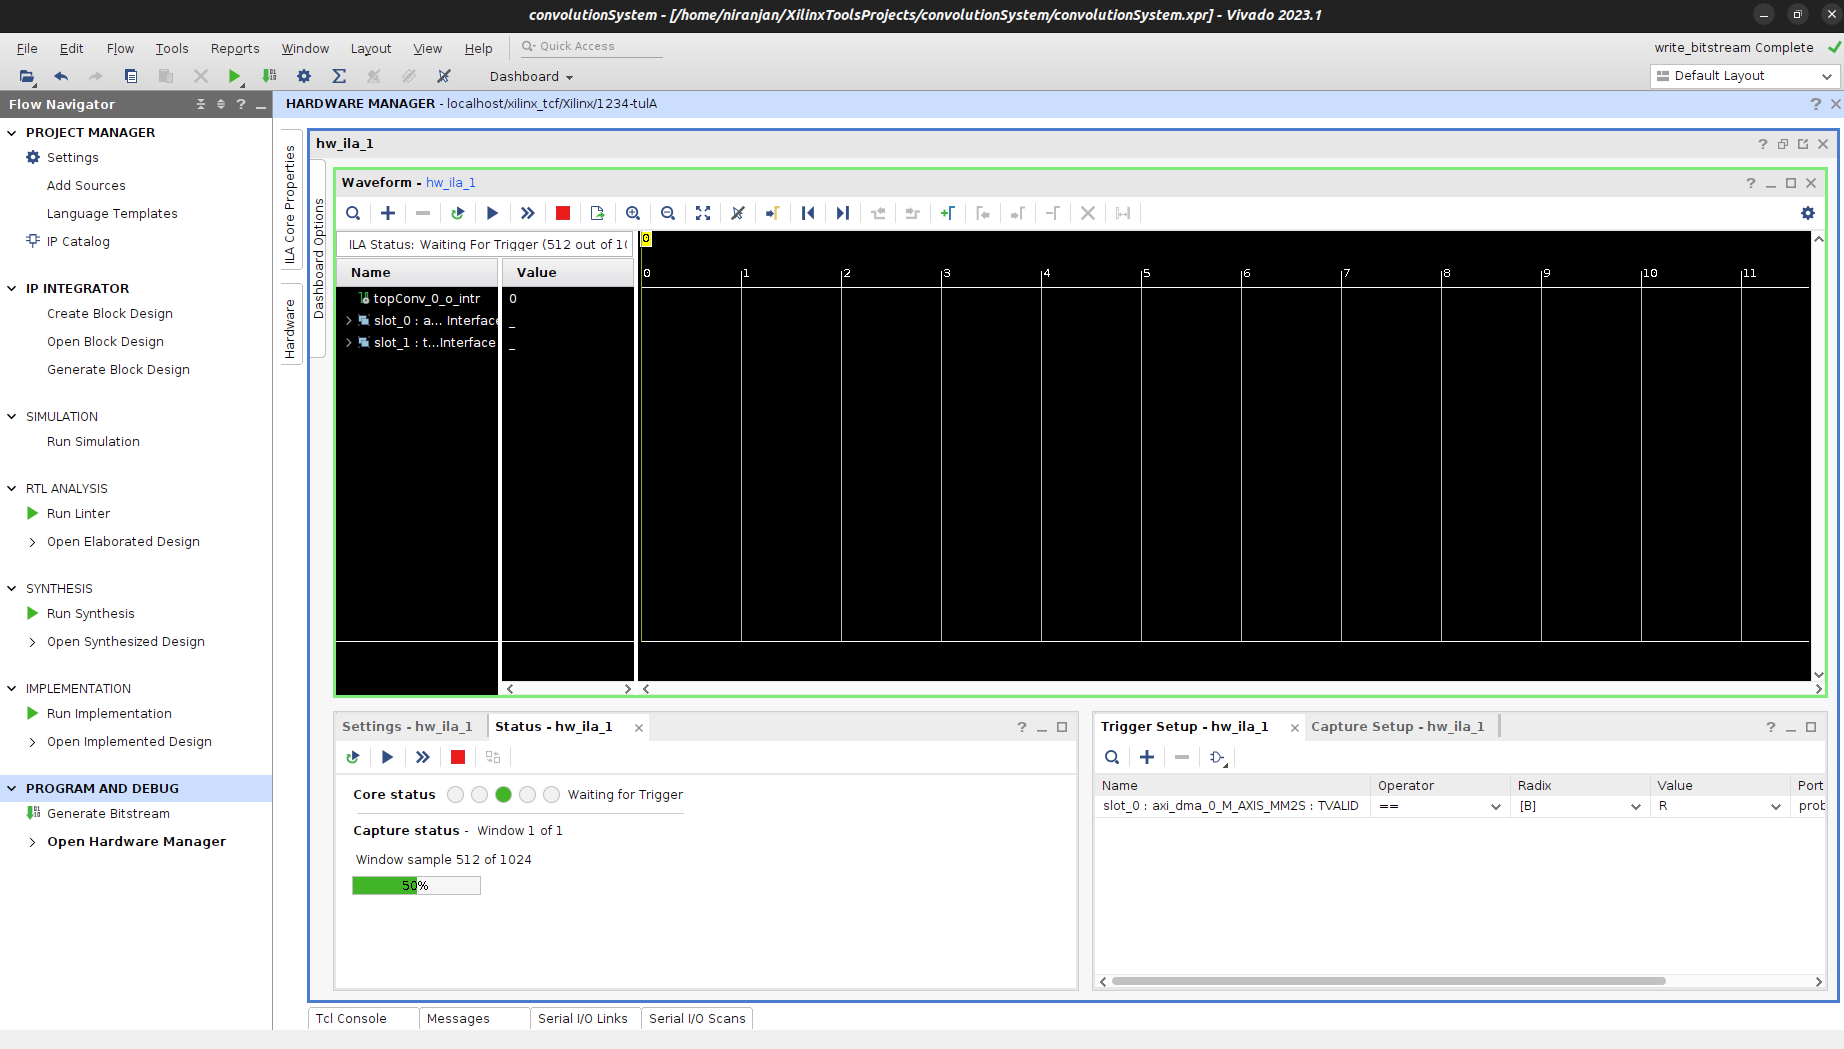
\includegraphics[width=0.87\linewidth]{images/dmaTrigger.png}
        \caption{Debug core waiting for DMA Image Data Valid}
        \label{fig:dmaTrigger}
    \end{figure}

    \begin{figure}[H]
        \centering
        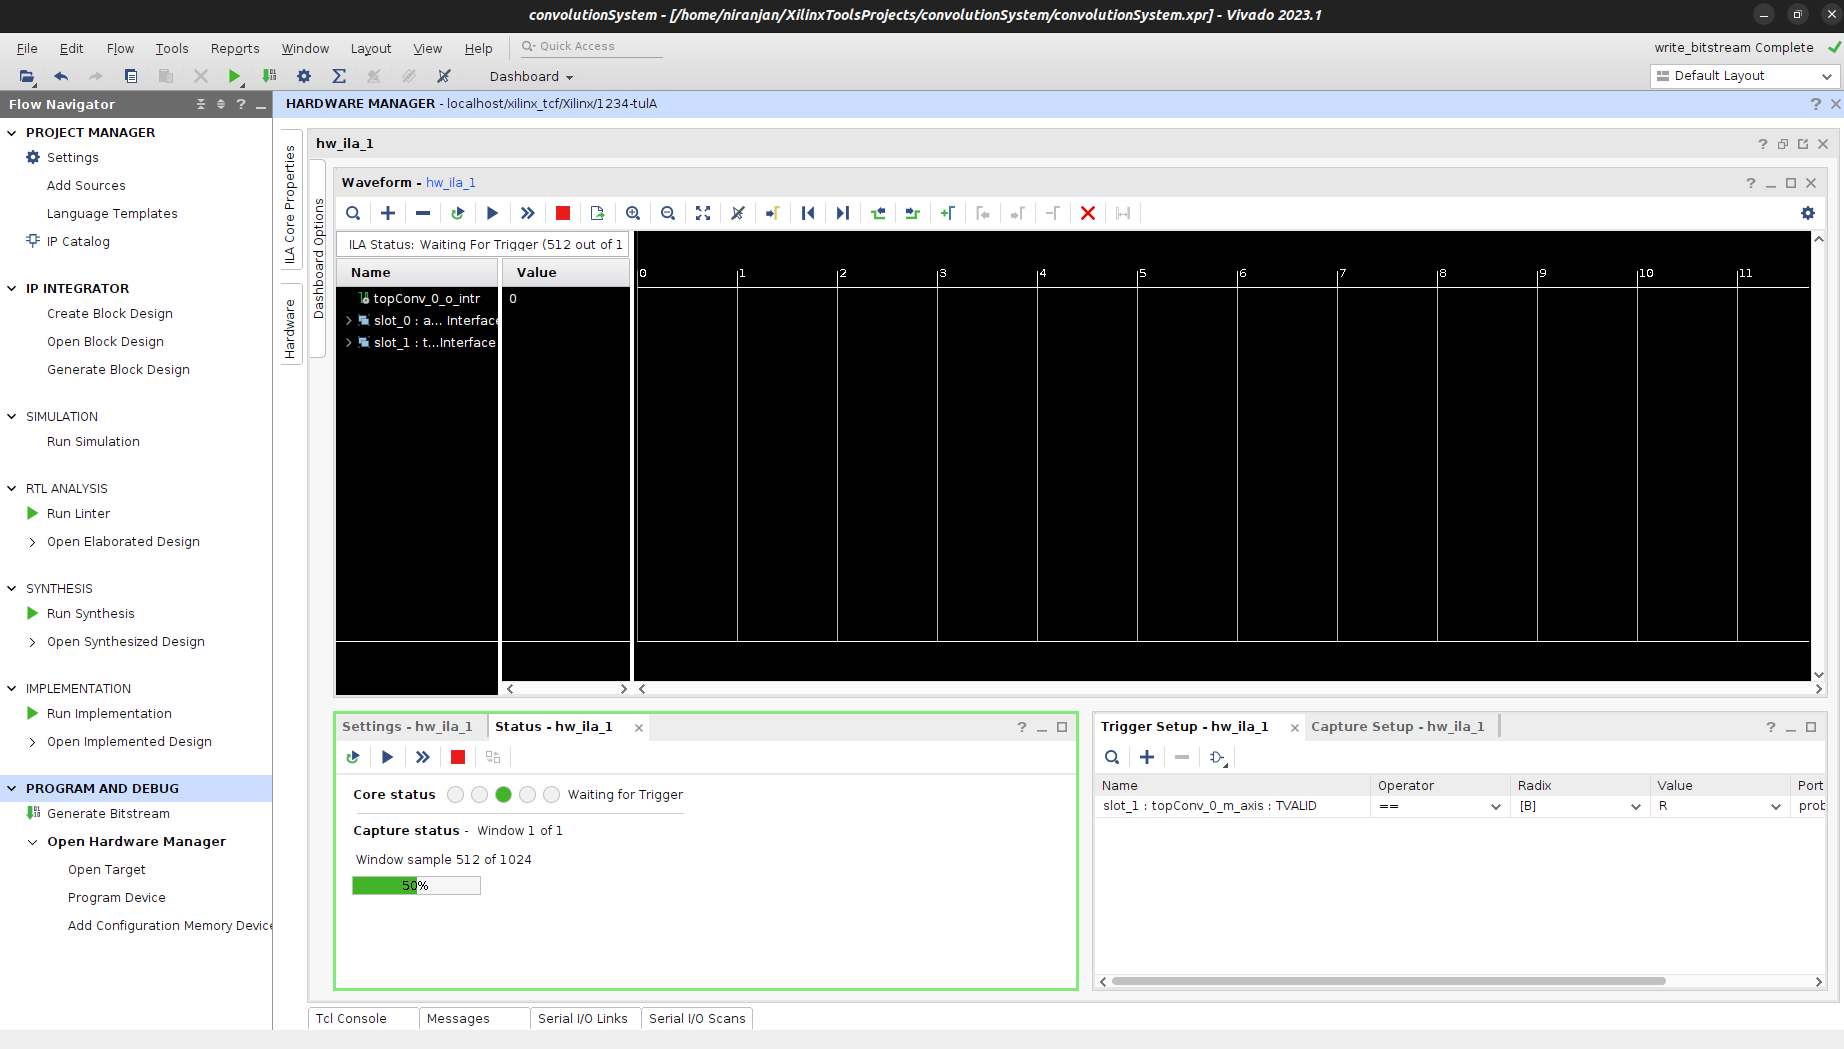
\includegraphics[width=0.87\linewidth]{images/convDataTrigger.png}
        \caption{Debug Core waiting for Convolution IP Output Data Valid}
        \label{fig:convDataTrigger}
    \end{figure}

    \begin{figure}[H]
        \centering
        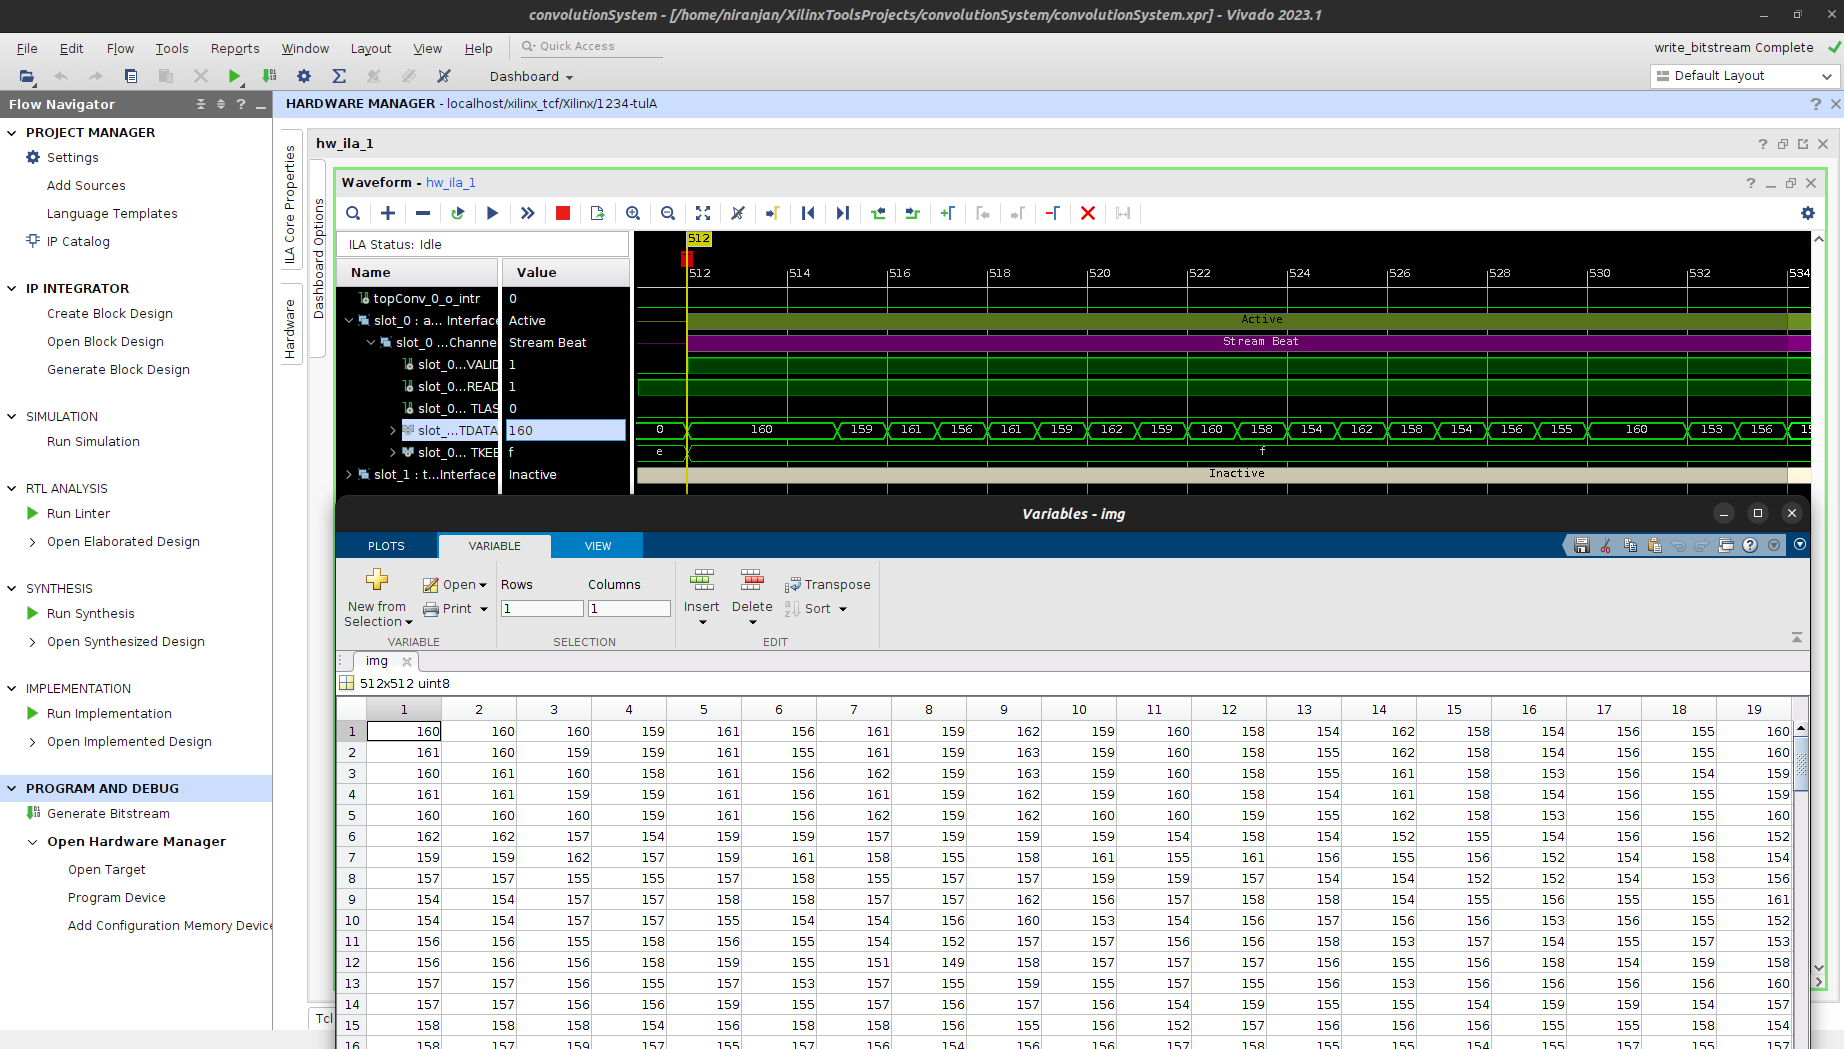
\includegraphics[width=1\linewidth]{images/imageDataTriggered.png}
        \caption{Image Data samples captured after DMA valid signal is triggered}
        \label{fig:imageDataTriggered}
    \end{figure}

    \begin{figure}[H]
        \centering
        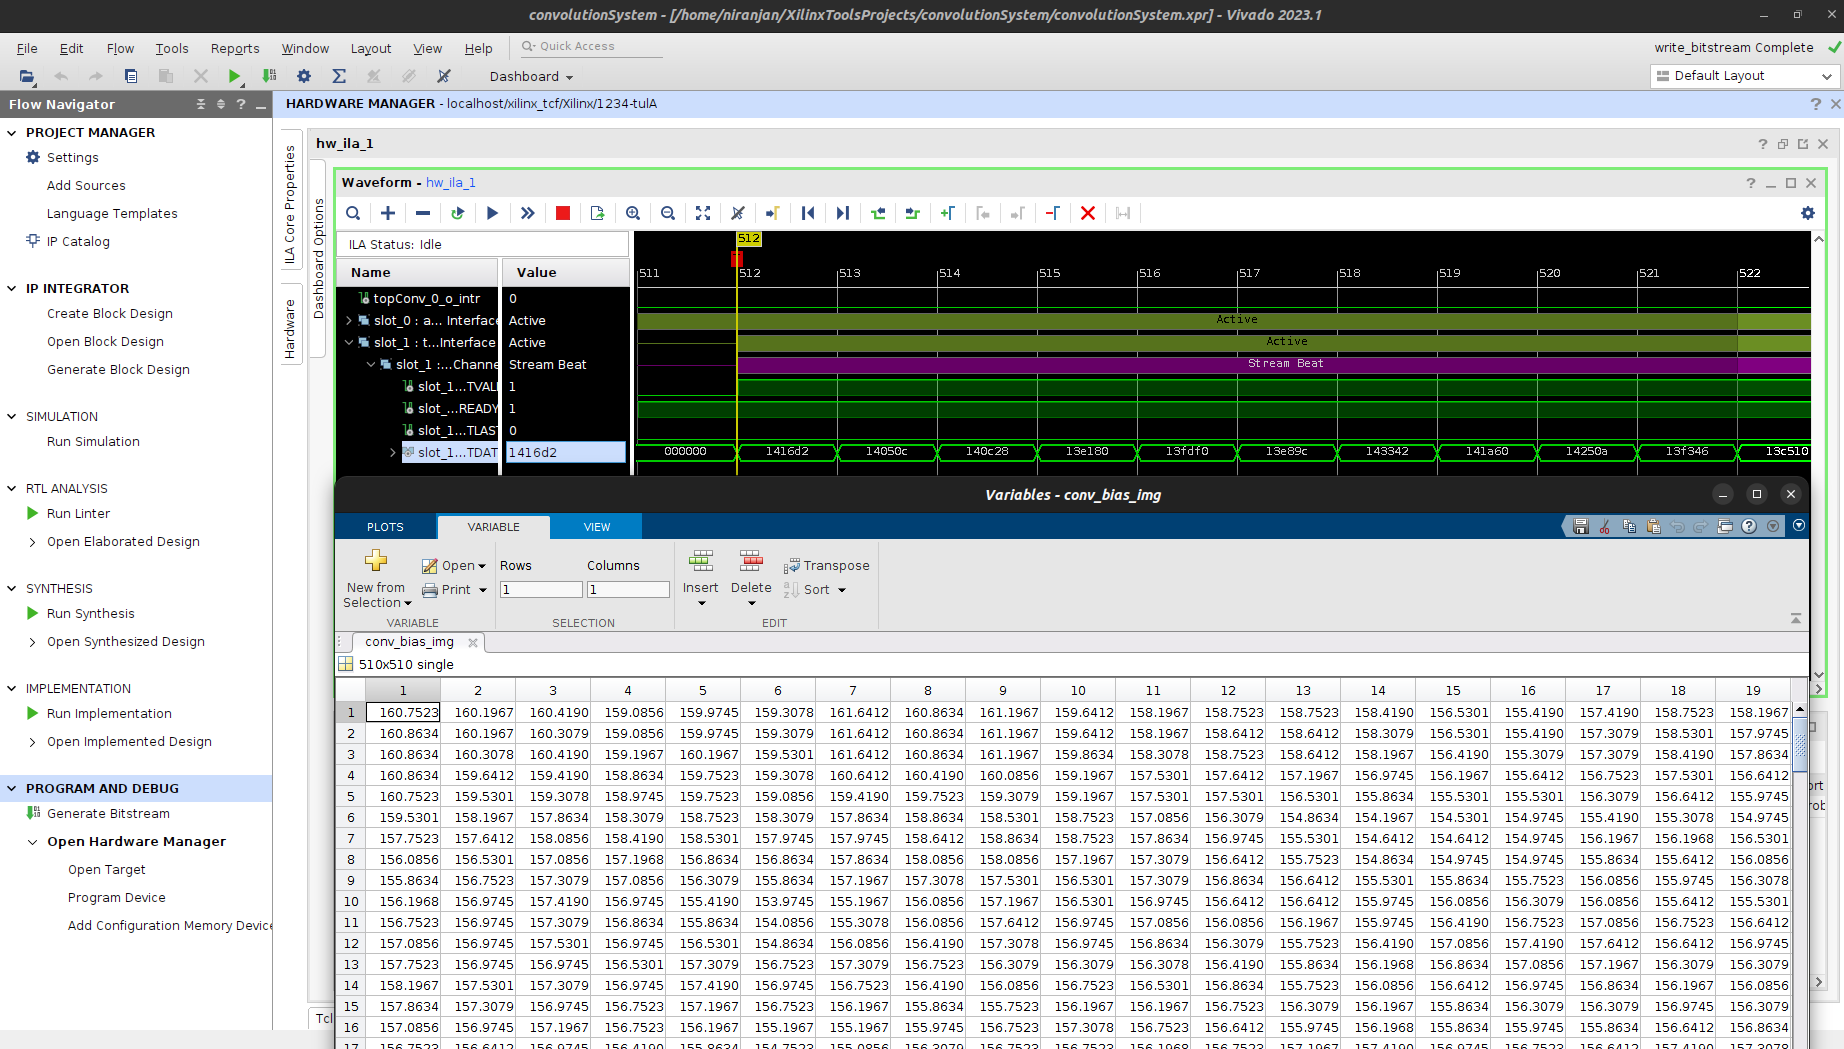
\includegraphics[width=1\linewidth]{images/convResultTriggered.png}
        \caption{Convolution Data samples captured after Convolution IP valid is triggered}
        \label{fig:convResultTriggered}
    \end{figure}

    \noindent
    Figure \ref{fig:imageDataTriggered} shows the captured data after the DMA's valid signal goes low-to-high. The same window contains a MATLAB window, which shows image data in uint8 format. The data captured is the first row of the image, and thus, it can be verified that proper data is being received by the convolution logic module by observing received and actual image pixel data on the waveform and MATLAB window.
    
    \noindent
    Figure \ref{fig:convResultTriggered} shows the output data captured by the debug core when the valid signal of the convolution IP goes from low to high. The data received results from a convolution operation performed on the first three rows for the initial few windows. Table \ref{tab:convDebugWaveform} shows equivalent decimal numbers corresponding to received hexadecimal data and expected convolution output data. The debug window has no option to convert data to a comparable form, thus, conversion is to be performed manually.
    \par \noindent
    The kernel and the bias used for the convolution operation at the hardware level are as follows.
    \begin{center}
    \begin{tabular}{|c|c|c|}
    \hline
    1/9 & 1/9 & 1/9 \\ \hline
    1/9 & 1/9 & 1/9 \\ \hline
    1/9 & 1/9 & 1/9 \\ \hline
    \end{tabular}
    \end{center}

    \[
    \text{bias} = 0.6411843299865723
    \]
    
    \par \noindent
    (Note initially 13 bits were used for fraction bits, but later on it was found that the integer part requires at least 3 bits thus, at a later stage, 12 bits of fraction and 3 bits of integer were adopted.)

    \begin{table}[H]
    \centering
    \renewcommand{\arraystretch}{1.3} % increases row height for better spacing
    \begin{tabular}{|c|c|c|}
    \hline
    \textbf{Convolution Output} & \textbf{Fixed Point Standard} & \textbf{MATLAB Reference} \\
    \textbf{(Hexadecimal)} & \textbf{Equivalent} & \textbf{Data} \\
    \hline
    1416d2 & 160.713134765625 & 160.75230 \\
    14050c & 160.15771484375  & 160.19673 \\
    140c28 & 160.3798828125   & 160.41896 \\
    13e180 & 159.046875        & 159.08563 \\
    13fdf0 & 159.935546875     & 159.97452 \\
    13e89c & 159.26904296875   & 159.30785 \\
    143342 & 161.601806640625  & 161.64117 \\
    141a60 & 160.82421875      & 160.86342 \\
    14250a & 161.157470703125  & 161.19675 \\
    13f246 & 159.571044921875  & 159.64119 \\
    \hline
    \end{tabular}
    \caption{Convolution Outputs Compared with MATLAB Reference Data}
    \label{tab:convDebugWaveform}
    \end{table}

    \noindent
    Thus, the appropriate image data is transferred to the Convolution IP, and the corresponding appropriate convolution output is also obtained. Due to fixed-point representation, the data suffers from loss of precision.

    \newpage
    
    

    

    